\section{\label{sec:evaluation}Evaluation}

\begin{table*}[h]
\centering
\small
\setlength{\tabcolsep}{5pt}
\renewcommand{\arraystretch}{1.12}
\begin{tabular}{
l l
S[table-format=2.1]
S[table-format=2.1]
S[table-format=2.1]
S[table-format=2.1]
S[table-format=2.1]
S[table-format=2.1]
}
\toprule
\textbf{LLM} & \textbf{Method}
& \multicolumn{3}{c}{\textbf{IMO-AnswerBench}}
& \multicolumn{3}{c}{\textbf{HLE}} \\
\cmidrule(lr){3-5}
\cmidrule(lr){6-8}
&
& {\textbf{NComm} $\downarrow$}
& {\textbf{Tok} $\mathbf{(\times 10^3)}$ $\downarrow$}
& {\textbf{Acc} $\uparrow$}
& {\textbf{NComm} $\downarrow$}
& {\textbf{Tok} $\mathbf{(\times 10^3)}$ $\downarrow$}
& {\textbf{Acc} $\uparrow$} \\
\midrule

\multirow{5}{*}{GPT-OSS-120B}
& \cellcolor{rowgray}Self Consistency
& \cellcolor{rowgray}0.0 & \cellcolor{rowgray}45.4 & \cellcolor{rowgray}36.7
& \cellcolor{rowgray}0.0 & \cellcolor{rowgray}14.1 & \cellcolor{rowgray}13.9 \\
& \cellcolor{white}GroupDebate
& \cellcolor{white}19.4 & \cellcolor{white}164.1 & \cellcolor{white}41.8
& \cellcolor{white}18.4 & \cellcolor{white}111.0 & \cellcolor{white}20.2 \\
& \cellcolor{rowgray}SID-ET
& \cellcolor{rowgray}17.5 & \cellcolor{rowgray}85.5 & \cellcolor{rowgray}38.7
& \cellcolor{rowgray}12.8 & \cellcolor{rowgray}39.6 & \cellcolor{rowgray}17.2 \\
& \cellcolor{white}S$^2$-MAD
& \cellcolor{white}22.8 & \cellcolor{white}131.4 & \cellcolor{white}42.1
& \cellcolor{white}14.0 & \cellcolor{white}67.7 & \cellcolor{white}21.0 \\
& \cellcolor{rowgray}\sysname
& \cellcolor{rowgray}{\bfseries 5.6} & \cellcolor{rowgray}{\bfseries 82.1} & \cellcolor{rowgray}{\bfseries 42.8}
& \cellcolor{rowgray}{\bfseries 7.3} & \cellcolor{rowgray}{\bfseries 39.1} & \cellcolor{rowgray}{\bfseries 21.4} \\

\midrule

\multirow{5}{*}{DeepSeek-V3.1}
& \cellcolor{white}Self Consistency
& \cellcolor{white}0.0 & \cellcolor{white}20.2 & \cellcolor{white}31.8
& \cellcolor{white}0.0 & \cellcolor{white}9.8 & \cellcolor{white}14.1 \\
& \cellcolor{rowgray}GroupDebate
& \cellcolor{rowgray}19.8 & \cellcolor{rowgray}234.6 & \cellcolor{rowgray}40.1
& \cellcolor{rowgray}19.6 & \cellcolor{rowgray}108.7 & \cellcolor{rowgray}14.9 \\
& \cellcolor{white}SID-ET
& \cellcolor{white}20.0 & \cellcolor{white}103.0 & \cellcolor{white}33.8
& \cellcolor{white}16.6 & \cellcolor{white}33.7 & \cellcolor{white}14.1 \\
& \cellcolor{rowgray}S$^2$-MAD
& \cellcolor{rowgray}20.9 & \cellcolor{rowgray}154.7 & \cellcolor{rowgray}36.8
& \cellcolor{rowgray}18.7 & \cellcolor{rowgray}71.7 & \cellcolor{rowgray}{\bfseries 16.7} \\
& \cellcolor{white}\sysname
& \cellcolor{white}{\bfseries 8.9} & \cellcolor{white}{\bfseries 91.7} & \cellcolor{white}{\bfseries 41.5}
& \cellcolor{white}{\bfseries 5.3} & \cellcolor{white}{\bfseries 30.3} & \cellcolor{white}{\bfseries 16.7} \\

\bottomrule
\end{tabular}
\vspace{3pt}
\caption{\textbf{\sysname achieves the best cost-accuracy tradeoff across all evaluated settings.} Evaluation results across two datasets and two LLMs.
% NComm, Tok, and Acc denote the number of cross-agent communications, the total token cost in thousands, and accuracy, respectively.
Arrows indicate whether higher ($\uparrow$) or lower ($\downarrow$) metric values are better. Best results are bold (NComm/Tok comparisons exclude Self Consistency, which is a no-debate reference).}
\label{tab:evaluation}
\vspace{-8pt}
\end{table*}

\noindent\textbf{Baselines.} We compare \sysname to (1) Self Consistency~\citep{Wang2023Self}, which aggregates independent agent solutions by majority vote without debate; (2) GroupDebate~\citep{Liu2025Groupdebate}, which restricts full-context exchange to random subgroups and allows only final-answer messages across groups; (3) SID-ET~\citep{Chen2025Sid}, which uses token log-likelihood-based self-confidence to select agents for debate; and (4) S$^2$-MAD~\citep{Zeng2025S2Mad}, which prunes communication links between agents with similar answers or response embeddings. All methods use the same pre-debate responses per question.

\noindent\textbf{Metrics.} We capture the tradeoff between communication cost and accuracy using three metrics: (1) number of communications (NComm), which counts pairwise context transfers in the abstract communication graph;
%\minghao{which serves as a proxy for communication complexity};
(2) total tokens, which captures the concrete overhead under specific model, dataset, and prompt settings; and (3) accuracy.
% Together, these metrics quantify the communication-accuracy tradeoff at both the protocol and implementation levels.

\noindent\textbf{MAD setting.} We use 6 agents per problem. All methods run for at most two debate rounds and may terminate after round one if at least five agents reach a clear consensus, thereby avoiding unnecessary cost inflation.

\noindent\textbf{LLMs and datasets.} We evaluate on GPT-OSS-120B and DeepSeek-V3.1 using IMO-AnswerBench and a filtered HLE~\citep{Phan2026Benchmark} subset containing only text-only, non-math, multiple-choice questions. This filtering ensures compatibility with GPT-OSS-120B (text-only LLM), avoids domain overlap with IMO-AnswerBench, and enables automatic correctness evaluation. We skip questions where all six agents share a unanimous answer before debate.

\noindent\textbf{Additional experimental settings.} We include other experimental details in Appendix~\ref{sec:additional-exp-setting}.

\subsection{Main results}

\noindent\textbf{\sysname achieves the best cost-accuracy tradeoff across all evaluated settings.} \sysname matches or exceeds every MAD baseline on accuracy while reducing per-question communications by 48–75\% and total tokens by 38–61\%, relative to the most accurate MAD baseline. On three of the four settings, \sysname strictly improves accuracy, with gains of up to 1.8, 7.7, and 4.7 points compared to GroupDebate, SID, and S$^2$-MAD, respectively. On DeepSeek-V3.1/HLE, \sysname matches S$^2$-MAD's accuracy but uses 72\%/58\% fewer communications/tokens per question.

\begin{figure}
\centering
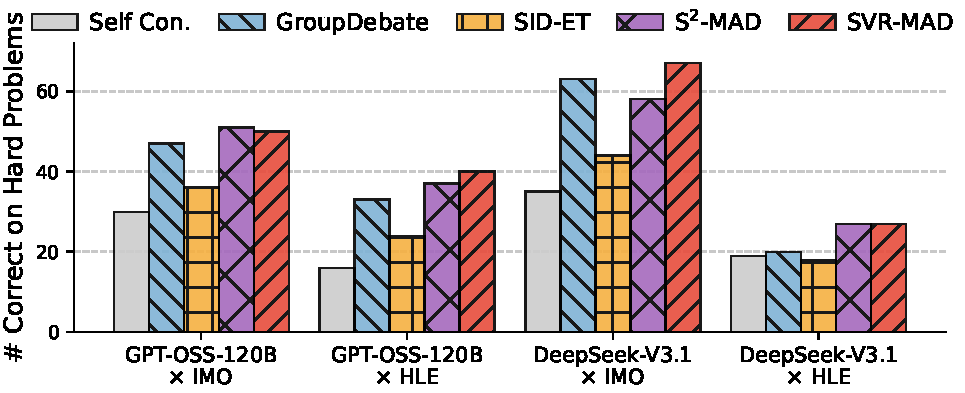
\includegraphics[width=0.9\columnwidth]{figures/tail-acc}
\caption{\label{fig:tail-acc} \textbf{\sysname achieves high accuracy on hard problems across all evaluated settings.} Accuracy of each method on problems where the number of correct agents before debate is within 1-3.}
\end{figure}


\noindent\textbf{\sysname achieves robust accuracy on hard problems while remaining cost-efficient.} Figure~\ref{fig:tail-acc} shows the number of hard problems each method answers correctly, where hard problems have 1--3 correct agents before debate. \sysname matches or exceeds all baselines on three of four settings, trailing only by one question to S$^2$-MAD on GPT-OSS/IMO. As S$^2$-MAD incurs 1.4--2.5$\times$ higher token cost on these hard problems, \sysname remains the most robust and cost-efficient.

\noindent\textbf{Ablation studies.} Appendix~\ref{sec:ablation} isolates the contribution of SVR by replacing it with alternative posterior signals in Algorithm~\ref{alg:sysname}. SVR improves accuracy by up to 8.75 points at matched token cost compared to the best alternative, showing that SVR provides an effective posterior signal beyond the benefits of the communication control flow.
